\documentclass[
  bibliography=totoc,     % Literatur im Inhaltsverzeichnis
  captions=tableheading,  % Tabellenüberschriften
  titlepage=firstiscover, % Titelseite ist Deckblatt
]{scrartcl}

% Warnung, falls nochmal kompiliert werden muss
\usepackage[aux]{rerunfilecheck}

% unverzichtbare Mathe-Befehle
\usepackage{amsmath}
% viele Mathe-Symbole
\usepackage{amssymb}
% Erweiterungen für amsmath
\usepackage{mathtools}

% Fonteinstellungen
\usepackage{fontspec}
% Latin Modern Fonts werden automatisch geladen
% Alternativ zum Beispiel:
%\setromanfont{Libertinus Serif}
%\setsansfont{Libertinus Sans}
%\setmonofont{Libertinus Mono}

% Wenn man andere Schriftarten gesetzt hat,
% sollte man das Seiten-Layout neu berechnen lassen
\recalctypearea{}

% deutsche Spracheinstellungen
\usepackage[ngerman]{babel}


\usepackage[
  math-style=ISO,    % ┐
  bold-style=ISO,    % │
  sans-style=italic, % │ ISO-Standard folgen
  nabla=upright,     % │
  partial=upright,   % │
  mathrm=sym,        % ┘
  warnings-off={           % ┐
    mathtools-colon,       % │ unnötige Warnungen ausschalten
    mathtools-overbracket, % │
  },                       % ┘
]{unicode-math}

% traditionelle Fonts für Mathematik
\setmathfont{Latin Modern Math}
% Alternativ zum Beispiel:
%\setmathfont{Libertinus Math}

\setmathfont{XITS Math}[range={scr, bfscr}]
\setmathfont{XITS Math}[range={cal, bfcal}, StylisticSet=1]

% Zahlen und Einheiten
\usepackage[
  locale=DE,                   % deutsche Einstellungen
  separate-uncertainty=true,   % immer Unsicherheit mit \pm
  per-mode=symbol-or-fraction, % / in inline math, fraction in display math
]{siunitx}

% chemische Formeln
\usepackage[
  version=4,
  math-greek=default, % ┐ mit unicode-math zusammenarbeiten
  text-greek=default, % ┘
]{mhchem}

% richtige Anführungszeichen
\usepackage[autostyle]{csquotes}

% schöne Brüche im Text
\usepackage{xfrac}

% Standardplatzierung für Floats einstellen
\usepackage{float}
\floatplacement{figure}{htbp}
\floatplacement{table}{htbp}

% Floats innerhalb einer Section halten
\usepackage[
  section, % Floats innerhalb der Section halten
  below,   % unterhalb der Section aber auf der selben Seite ist ok
]{placeins}

% Seite drehen für breite Tabellen: landscape Umgebung
\usepackage{pdflscape}

% Captions schöner machen.
\usepackage[
  labelfont=bf,        % Tabelle x: Abbildung y: ist jetzt fett
  font=small,          % Schrift etwas kleiner als Dokument
  width=0.9\textwidth, % maximale Breite einer Caption schmaler
]{caption}
% subfigure, subtable, subref
\usepackage{subcaption}

% Grafiken können eingebunden werden
\usepackage{graphicx}

% schöne Tabellen
\usepackage{tabularray}
\UseTblrLibrary{booktabs, siunitx}

% longtblr-Umgebung auf Deutsch
\DefTblrTemplate{contfoot-text}{normal}{Weiter auf der nächsten Seite}
\SetTblrTemplate{contfoot-text}{normal}
\DefTblrTemplate{conthead-text}{normal}{(Fortsetzung)}
\SetTblrTemplate{conthead-text}{normal}

% Verbesserungen am Schriftbild
\usepackage{microtype}

% Literaturverzeichnis
\usepackage[
  backend=biber,
]{biblatex}
% Quellendatenbank
\addbibresource{lit.bib}
\addbibresource{programme.bib}

% Hyperlinks im Dokument
\usepackage[
  german,
  unicode,        % Unicode in PDF-Attributen erlauben
  pdfusetitle,    % Titel, Autoren und Datum als PDF-Attribute
  pdfcreator={},  % ┐ PDF-Attribute säubern
  pdfproducer={}, % ┘
]{hyperref}
% erweiterte Bookmarks im PDF
\usepackage{bookmark}

% Trennung von Wörtern mit Strichen
\usepackage[shortcuts]{extdash}
\usepackage{tikz}
\usepackage[european]{circuitikz}   
% Code Einbindung
\usepackage{xcolor}
\definecolor{LightGray}{gray}{0.9}
\usepackage{minted}
\setminted{
  autogobble,
  breaklines,
  stripnl=true,
  style=tango,
  baselinestretch=1.2,
  bgcolor=LightGray,
  fontsize=\footnotesize,
}

\author{%
  David Lohberg\\%
  \href{mailto:david.lohberg@tu-dortmund.de}{david.lohberg@tu-dortmund.de}%
  \and%
  Felix Michael Bernd Wendeln\\%
  \href{mailto:felix.wendeln@tu-dortmund.de}{felix.wendeln@tu-dortmund.de}%
}
\publishers{TU Dortmund – Fakultät Physik}

\usepackage{expl3}
\usepackage{xparse}

\usepackage{mleftright}
\setlength{\delimitershortfall}{-1sp}

\ExplSyntaxOn

\NewDocumentCommand \I {} { \symup{i} }
\NewDocumentCommand \E {} { \symup{e} }
\NewDocumentCommand \mpi {} { \symup{\pi} }

\NewDocumentCommand \dif {m} { \mathinner{\symup{d} #1} }
\NewDocumentCommand \Dif {m} { \mathinner{\symup{D} #1} }
\NewDocumentCommand \del {m} { \mathinner{\symup{\delta} #1} }
\NewDocumentCommand \Del {m} { \mathinner{\symup{\Delta} #1} }

\let\vaccent=\v % alten Befehl kopieren
\RenewDocumentCommand \v {} % Befehl überschreiben
  {
    \TextOrMath{
      \vaccent % Textmodus
    }{
      \symbf % Mathemodus
    }
  }

\AtBeginDocument{ % wird bei \begin{document} ausgeführt
  % werden sonst wieder von unicode-math überschrieben
  \RenewDocumentCommand \Re {} {\operatorname{Re}}
  \RenewDocumentCommand \Im {} {\operatorname{Im}}
}

\let\ltext=\l
\RenewDocumentCommand \l {}{ \TextOrMath{ \ltext }{ \mleft } }
\let\raccent=\r
\RenewDocumentCommand \r {}{ \TextOrMath{ \raccent }{ \mright } }

\DeclarePairedDelimiter{\abs}{\lvert}{\rvert}
\DeclarePairedDelimiter{\norm}{\lVert}{\rVert}

\DeclarePairedDelimiter{\bra}{\langle}{\rvert}
\DeclarePairedDelimiter{\ket}{\lvert}{\rangle}
% <name> <#arguments> <left> <right> <body>
\DeclarePairedDelimiterX{\braket}[2]{\langle}{\rangle}{#1 \delimsize| #2}


\NewDocumentCommand \OverfullCenter {+m} {
\noindent\makebox[\linewidth]{#1} }

\ExplSyntaxOff


\subject{VERSUCH 300}
\title{Oszilloskop}
\date{%
  Durchführung: 03.11.2026
  \hspace{3em}
  Abgabe: 10.11.2026
}
\usepackage{subcaption}
\usepackage[section, below]{placeins}
\usepackage[]{caption} % Captions schöner machen
\usepackage{comment}
\FloatBarrier

\begin{document}
\maketitle
\thispagestyle{empty}
\tableofcontents
\newpage

\section{Versuchsaufbau}
Für die folgenden Versuche werden folgende Bauteile in verschiedenen Weisen miteinander verbunden und eingestellt. 
Es werden ein analoges Oszilloskop, in diesem Fall ein HAMEG HM-205-3(\ref{fig:oszilloskop}), sowie eine Leiterplatte, hier das VELLEMAN - 
EDU06 Oszilloskop Lern Kit 839006(\ref{fig:bord}), benötigt. 
Mit einem Tastkopf werden die jeweiligen Signale abgegriffen und am Oszilloskop dargestellt.
\begin{figure}[H]
    \centering

    \begin{subfigure}{0.45\textwidth}
        \centering
        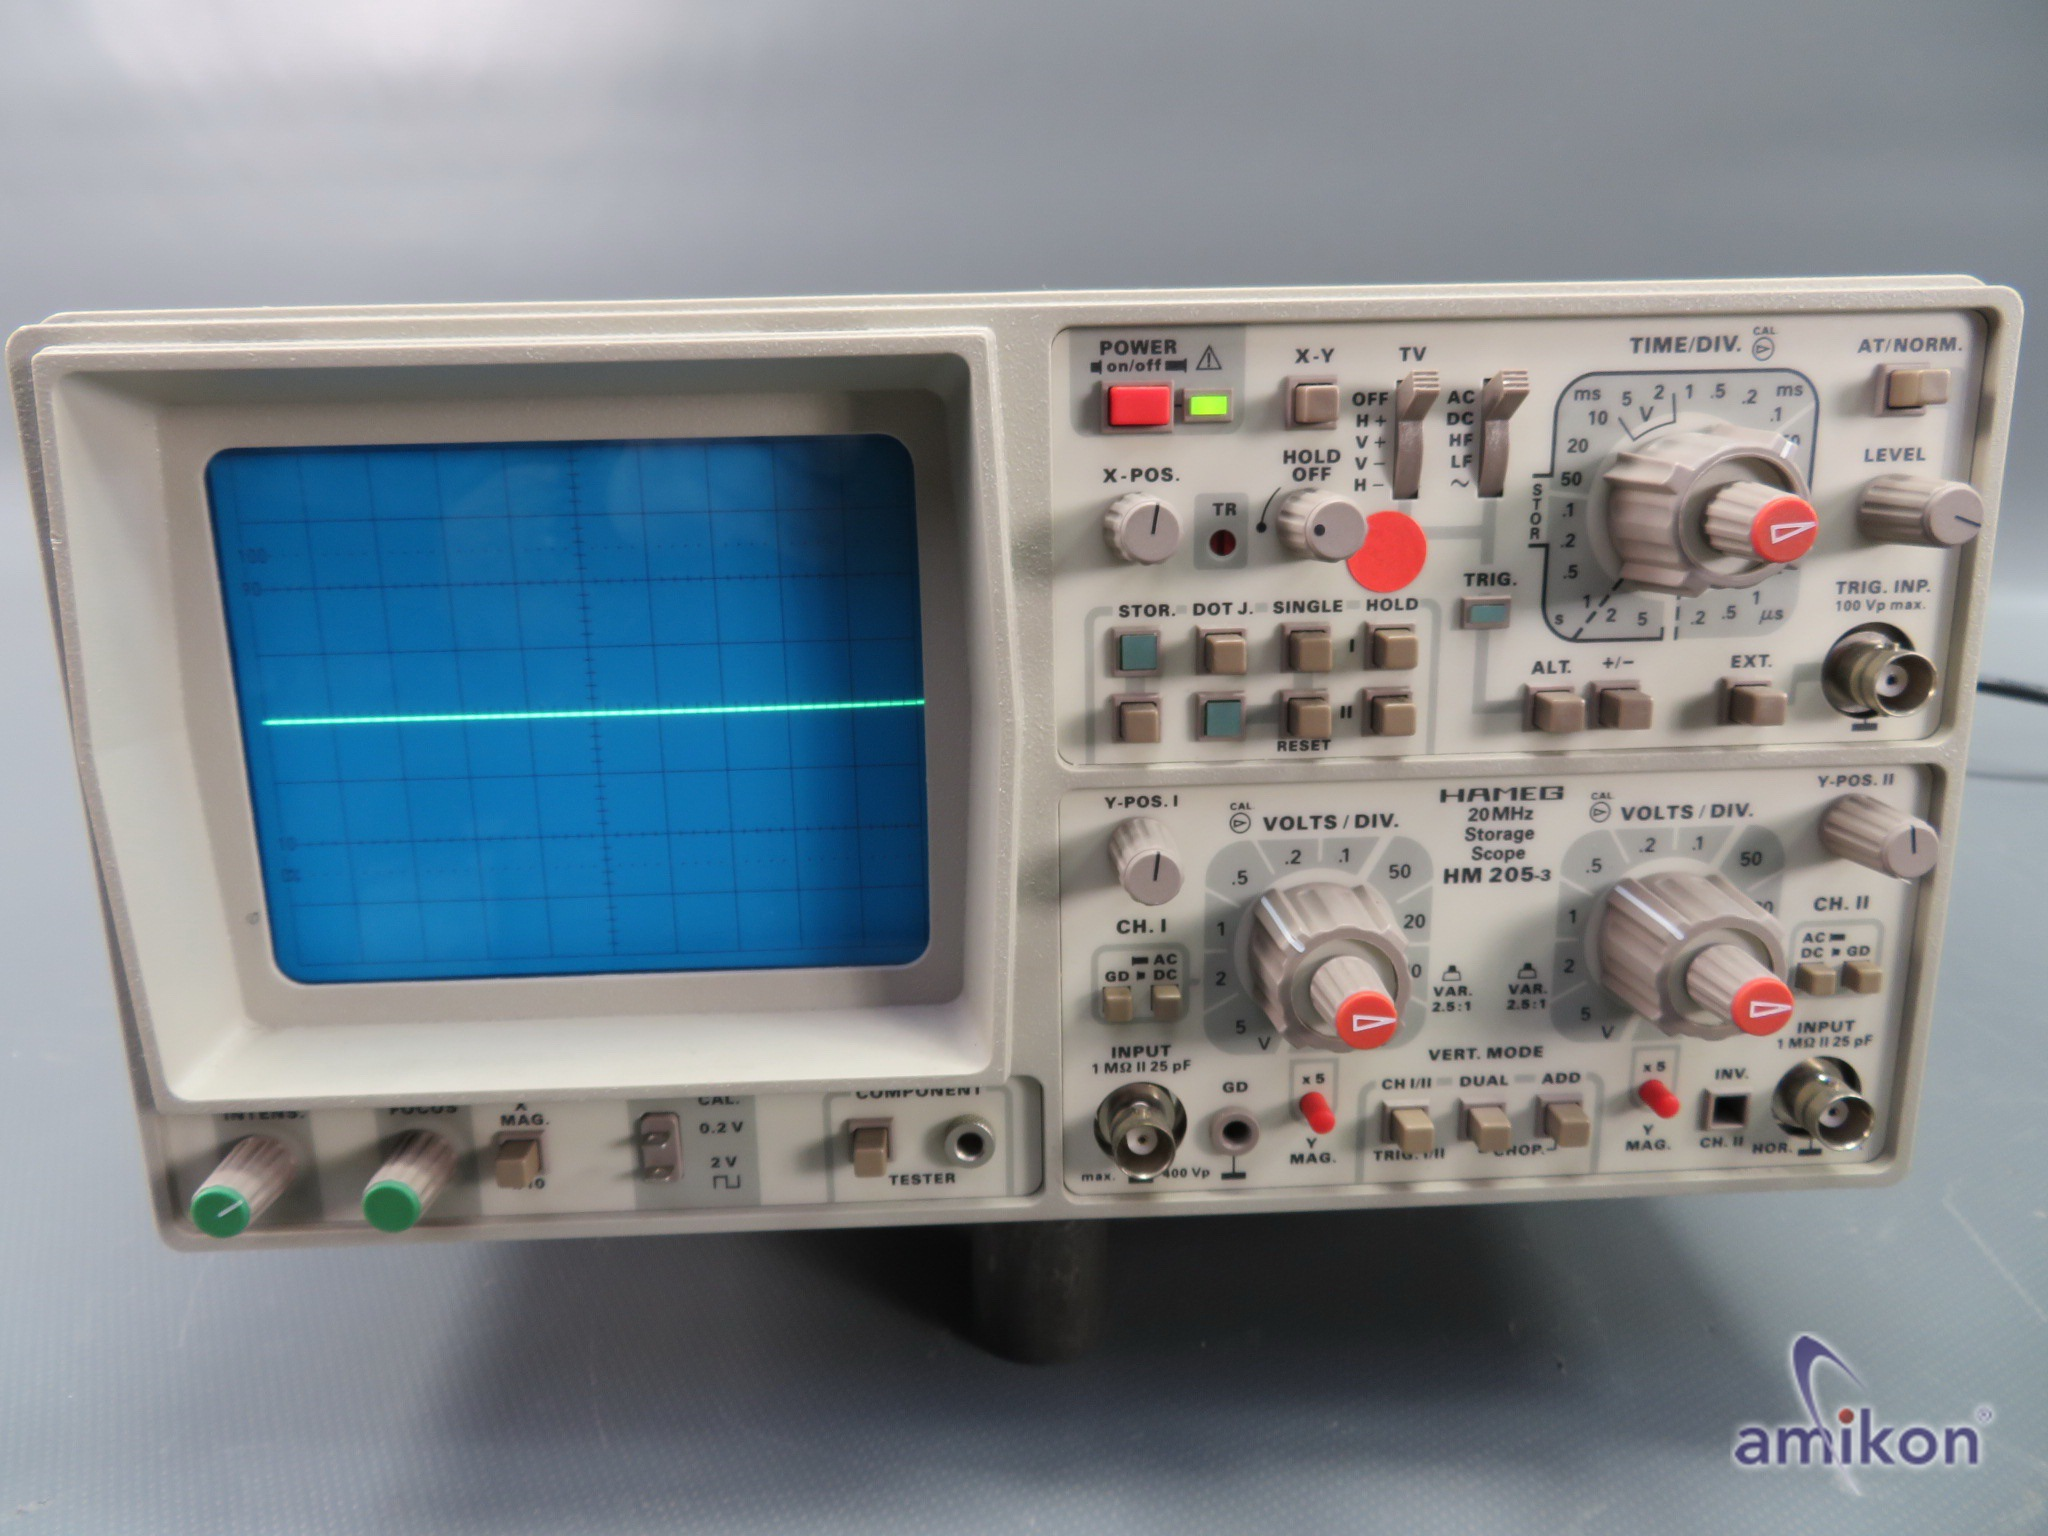
\includegraphics[width=\textwidth]{HAMEG-HM205-3.jpg}
        \caption{HAMEG Oszilloskop HM205-3\cite{Oszilloskop}}
        \label{fig:oszilloskop}
    \end{subfigure}
    \hfill
    \begin{subfigure}{0.45\textwidth}
        \centering
        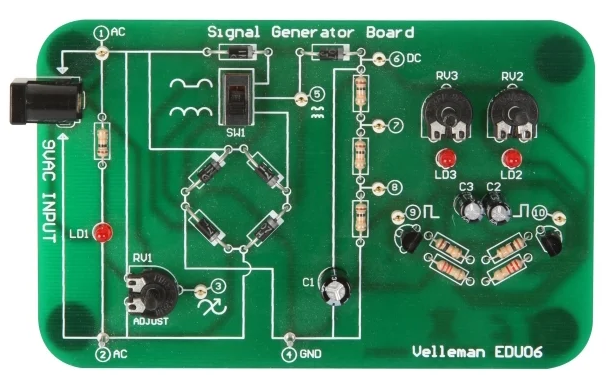
\includegraphics[width=\textwidth]{Bord.png}
        \caption{VELLEMAN-EDU06 Oszilloskop Lern Kit\cite{Bord}}
        \label{fig:bord}
    \end{subfigure}

\end{figure}
\section{Durchführung}
\subsection{Kalibrierung}
Bevor mit dem Oszilloskop experimentiert werden kann, muss es erstmal richtig kalibriert werden. 
Hierfür hat das Oszilloskop selbst einen Abgriff, der ein Blocksignal mit einer festen(0.2 V) Spannung und einer festen Frequenz abgibt,
welche aber nicht einsehbar war. Daher wurde die Kalibrierung von der Frequenz nach Signallänge gesetzt, während die Spannung ohne Einschränkungen kalibriert werden konnte.
Im Folgenden wurde die Kalibrierung nicht mehr angepasst.
\subsection{Messungen von Wechselstrom}
Für die Messungen des Wechselstroms wurde vom Generator Bord am Abgriff 1 das Signal abgegriffen, welches am Abgriff 2 geerdet wurde(\ref{fig:bord}). 
Zuerst wurde die Amplitude des Wechselstroms in verschiedenen Messbereichen gemessen. Da jedoch nur im höchsten Messbereich (5V/DIV) die Amplitude ablesbar war, musste für die weiteren Messungen ein Widerstand zwischengeschaltet werden, welcher das Signal um den Faktor 10 geteilt hat. Die Messung erfolgte in den Einstellungen 1,2,5 V/DIV und der festen Einstellung 2ms/DIV, wobei die Amplitude Peak-to-Peak gemessen wurde.

\noindent
Danach folgte die Messung mit variabler Amplitude, dafür wurde am Generator Bord am Abgriff 3 das Signal abgenommen, die Erdung erfolgt weiterhin am Abgriff 2(\ref{fig:bord}). Das sorgt dafür, dass ein Potentiometer RV1(\ref{fig:bord})
zwischengeschaltet wird.
Es wurden die Amplitude von der stärksten und vom schwächsten möglichen Signal gemessen(Peak-to-Peak), auch hier mit verschiedenen Messbereichen ($U_{min}$ in 0.2, 0.1 V/DIV und $U_{max}$ in 5,2 V/DIV) wobei bei der zweiten Messungen wieder ein 10x Widerstand zwischengeschaltet wird. 

\subsection{Einweg- und Zweiweggleichrichtung}
In diesem Teil des Versuchs werden Einweg- und Zweiweggleichrichtung sowie Unterschiede bei der AC bzw. DC Einstellung des Triggers auf dem Oszilloskop untersucht. Zunächst wird der Messkopf am Abgriff 5 angeschlossen und an Abgriff 4 geerdet. Der Schalter SW1 der Leiterplatte wird in die obere Position, also in Einweggleichrichtung geschaltet. Es wird die Amplitude und Periodendauer am Oszilloskop gemessen. Danach wird dies mit SW1 in unterer Position, also der Zweiweggleichrichtung, wiederholt. Der Messbereich wird auf 2ms/DIV und 5V/DIV für die Erste, bzw. 1ms/DIV und 5V/DIV für die Zweite Messung eingestellt. Bei beiden ist der Trigger auf DC gestellt
(\ref{fig:bord}),(\ref{fig:oszilloskop}).

\noindent
Nun wird der Unterschied zwischen der Triggereinstellung AC und DC untersucht. Dafür wird der Messkopf auf den Abgriff 6 gestellt und bleibt an Abgriff 4 geerdet. Die Einstellungen 2ms/DIV und 0,5V/DIV mit SW1 nach oben geschaltet werden gewählt. Anschließend wird der Knopf GD gedrückt und die entstehende 0V Linie auf die x-Achse verschoben. Nach erneutem drücken des GD Knopfes wird der Abstand zur x-Achse gemessen. Dieser Vorgang wird für den Messkopf auf Abgriff 7 bzw. 8 wiederholt
(\ref{fig:bord}),(\ref{fig:oszilloskop}).

\noindent
Zuletzt wird bei gleichbleibendem Messbereich der Messkopf wieder am Abgriff 6 angebracht und der Trigger auf AC gestellt. Der SW1 Schalter wird zunächst auf Einweggleichrichtung und danach auf Zweiweggleichrichtung eingestellt. Bei beiden Malen wird die Amplitude gemessen
(\ref{fig:bord}),(\ref{fig:oszilloskop}).
\subsection{Messungen Anstiegszeit}
Um die variable Frequenz zu erhalten, wurde das Signal am Abgriff 9 gemessen und mit Abgriff 4 geerdet(\ref{fig:bord})
. Mit RV2 und RV3 kann die Frequenz eingestellt werden(\ref{fig:bord})
. Das Signal folgt in einer Puls-Pause-Sequenz, von dieser wurde die Anstiegszeit, welche ca. 90\% des Anstiegs darstellt, gemessen. Diese Messung wurde mit positiven und negativen Flanken wiederholt. Die Messung erfolgte in den Messbereichen 2ms/DIV und 2V/DIV. 

\printbibliography{}
\end{document}